%%%%%%%%%%%%%%%%%%%%%%%%%%%%%%%%%%%%%%%%%%%%%%%%%%%%%%%%%
%%             东南大学电路实验报告 LaTeX 模板
%%                SEU-Circuit-Report.cls
%% https://github.com/Teddy-van-Jerry/SEU_Circuit_Report
%% ======================================================
%% 版本信息:
%% v1.1 (Oct. 24, 2021)
%% ------------------------------------------------------
%% 模板制作:
%% Teddy van Jerry, (me@teddy-van-jerry.org)
%% * GitHub: https://github.com/Teddy-van-Jerry
%% * Website: https://teddy-van-jerry.org
%% * Blog: https://blog.teddy-van-jerry.org
%% ------------------------------------------------------
%% 使用说明:
%% 1. 编译使用 XeLaTeX 和 Biber
%% 2. 报告基本信息通过修改导言区以 exp 开头的命令
%% 3. 参考文献位于 ref/ref.bib
%% 4. 报告模板依据 MIT License 开源共享
%% ------------------------------------------------------
%% Copyright 2021 (c) Teddy van Jerry
%%
%% Permission is hereby granted, free of charge, to any
%% person obtaining a copy of this software and
%% associated documentation files (the "Software"), to
%% deal in the Software without restriction, including
%% without limitation the rights to use, copy, modify,
%% merge, publish, distribute, sublicense, and/or sell
%% copies of the Software, and to permit persons to whom
%% the Software is furnished to do so, subject to the
%% following conditions:
%%
%% The above copyright notice and this permission notice
%% shall be included in all copies or substantial
%% portions of the Software.
%% 
%% THE SOFTWARE IS PROVIDED "AS IS", WITHOUT WARRANTY OF
%% ANY KIND, EXPRESS OR IMPLIED, INCLUDING BUT NOT
%% LIMITED TO THE WARRANTIES OF MERCHANTABILITY, FITNESS
%% FOR A PARTICULAR PURPOSE AND NONINFRINGEMENT. IN NO
%% EVENT SHALL THE AUTHORS OR COPYRIGHT HOLDERS BE LIABLE
%% FOR ANY CLAIM, DAMAGES OR OTHER LIABILITY, WHETHER IN
%% AN ACTION OF CONTRACT, TORT OR OTHERWISE, ARISING
%% FROM, OUT OF OR IN CONNECTION WITH THE SOFTWARE OR THE
%% USE OR OTHER DEALINGS IN THE SOFTWARE.
%%%%%%%%%%%%%%%%%%%%%%%%%%%%%%%%%%%%%%%%%%%%%%%%%%%%%%%%%%

%% 使用实验报告模板类(字体大小 12pt 最适合)
\documentclass[12pt]{SEU-Circuit-Report}

%%%%%%%%%%%%%%%%%%%% 报告基本信息 %%%%%%%%%%%%%%%%%%%%
\expno{3} % 实验序号
\expname{应用Multisim软件工具设计电路验证网络定理} % 实验名称
\exphouse{TVJ Group} % 学院
\expmajor{\LaTeX\ Design} % 专业
\expauthor{Teddy van Jerry} % 姓名
\expID{123456} % 学号
\explab{} % 实验室
\expgroup{} % 实验组别
\expmates{} % 同组人员
\expdate{2021年10月19日} % 实验日期
\expgrade{} % 成绩评定
\exptutor{Mentor Name} % 评阅老师
%%%%%%%%%%%%%%%%%%%%%%%%%%%%%%%%%%%%%%%%%%%%%%%%%%%%

%% 报告正文
\begin{document}
    % 打印封面页
    \exptitlepage

    \section{实验目的}
        \begin{enumerate}
            \item 通过实验加深对参考方向、基尔霍夫定理、叠加定理、戴维南定理的理解; 
            \item Multisim 软件入门:元器件配置、电路连接、电路参数测试; 
            \item 通过学习对实验结果的分析对比,了解虚拟仿真与实物实验的差异。
        \end{enumerate}

    \section{实验原理}
        \begin{enumerate}
            \item Multisim 仿真软件;
            \item \textbf{基尔霍夫定理}包括电流定律(KCL)和电压定律(KVL),用公式表示为 $\sum I=0$ 和 $\sum V=0$。KCL 即流入节点电流等于流出电流,KVL 即环路一周电势降为零;
            \item \textbf{叠加定理}:在线性电路中,任一支路的电流或电压等于电路中每一个激励源单独作用 (令其他激励源为零值)时,在该支路所产生的电流或电压的代数和。注意:不考虑电流源时即将电流源被短路,考虑电压源则是将电压源断路;
            \item \textbf{戴维南定理}(Thevenin's theorem)说明了线性含源单端口网络对外电路可等效于一个电压源串联一个电阻\cite{circuit_book},这次试验直接用到的是两个电压源并联的公式
            \begin{equation}\label{eq:thevenin}
                U=\frac{r_1U_2+r_2U_1}{r_1+r_2},
            \end{equation}
            式中 $r_{1,2}$ 分别为 $U_{1,2}$ 支路上的电阻值。而电阻即去掉电压源后的并联电阻。
        \end{enumerate}

    \section{实验内容}

        \subsection{基尔霍夫定理、叠加定理的验证}\label{subsec:exp1}
            (1) 按图~\ref{fig:1init}~所示实验电路建立电路。按表~\ref{tab:1data}~用电压表和电流表测量各电阻两端电压和各支路电流。分析说明测量结果。
            \begin{figure}[htbp]
                \centering
                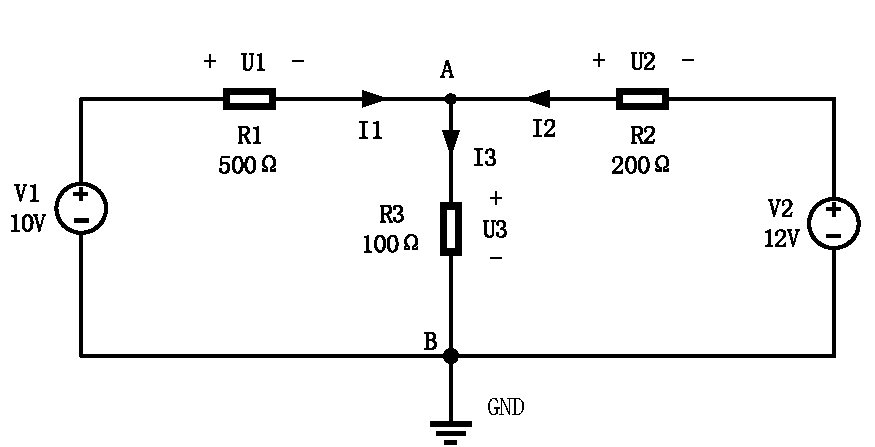
\includegraphics[width=.8\linewidth]{fig/实验电路1.pdf}
                \caption{实验电路}
                \label{fig:1init}
            \end{figure}
            \begin{figure}[htbp]
                \centering
                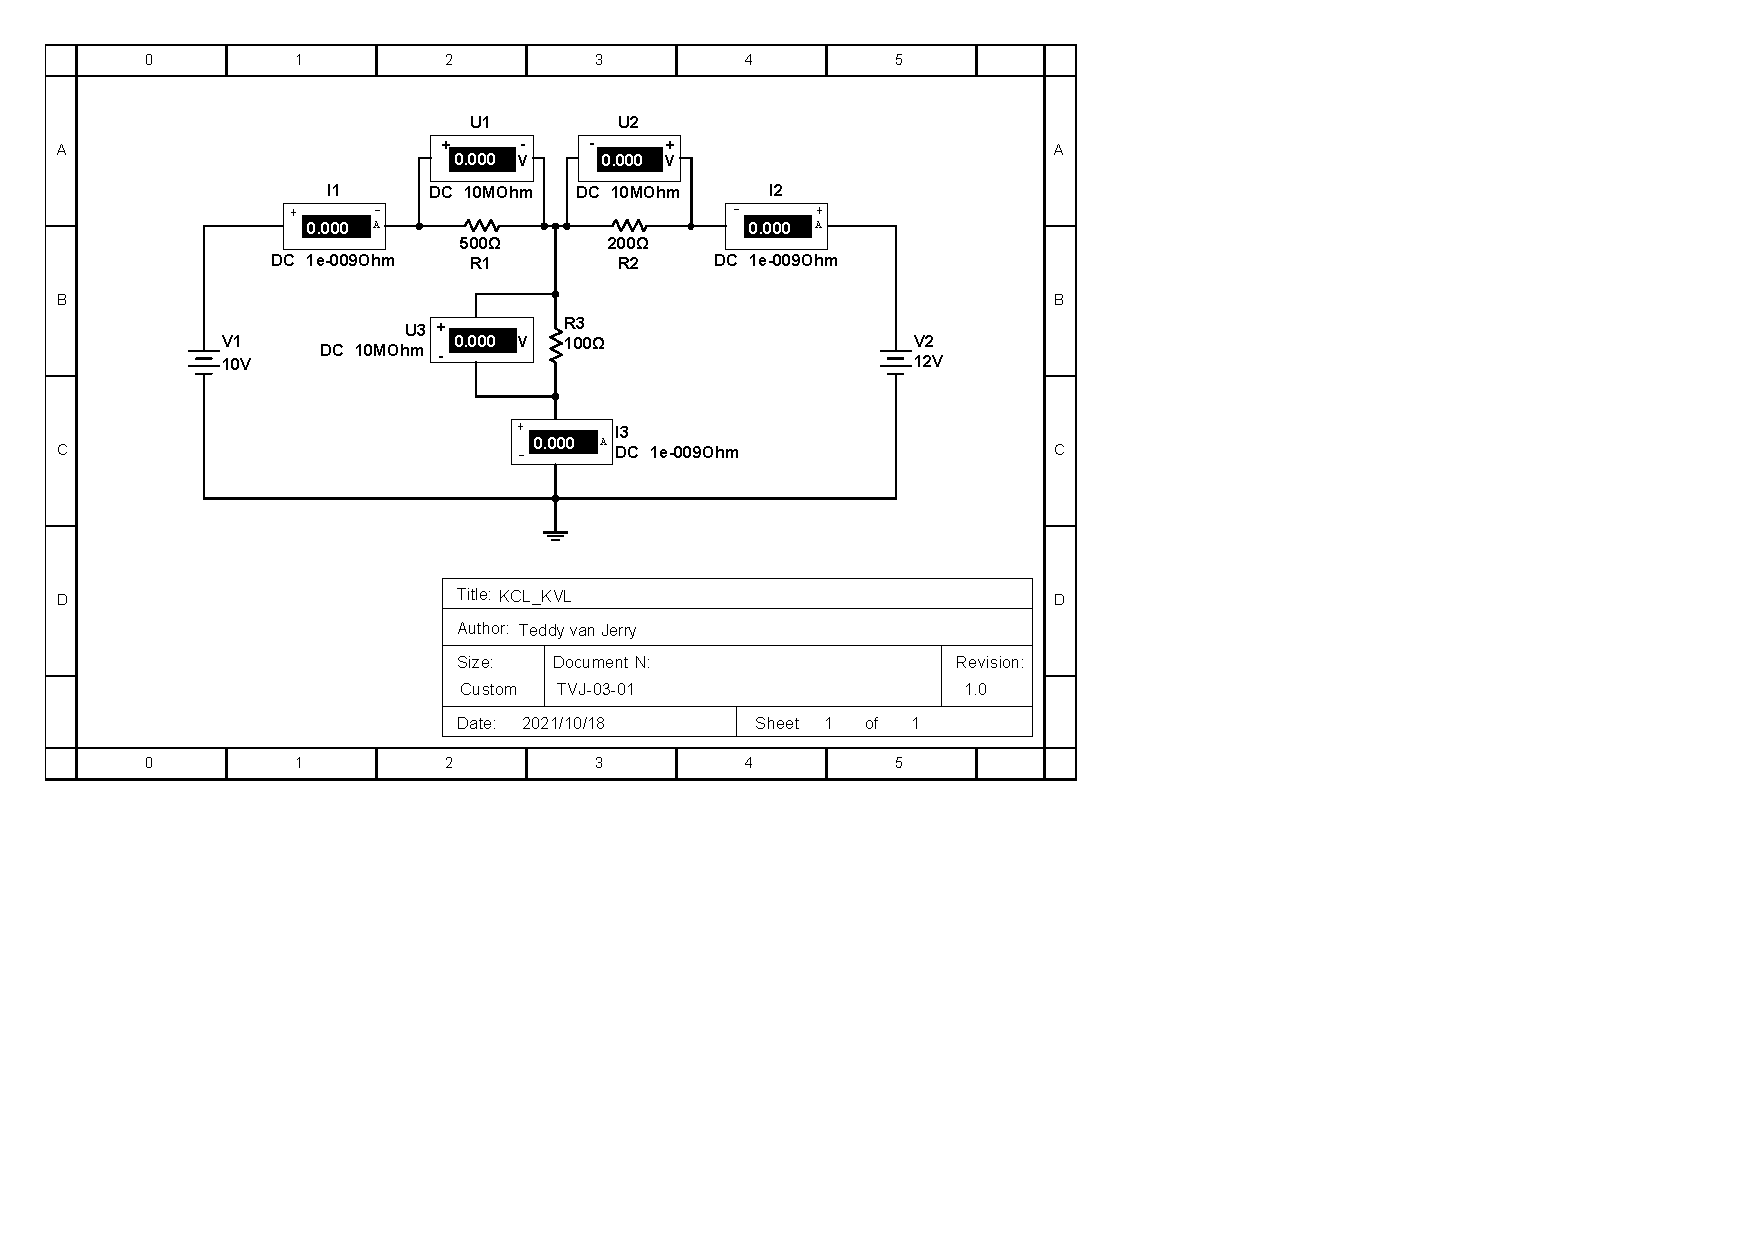
\includegraphics[width=.8\linewidth]{KCL_KVL.pdf}
                \caption{仿真电路图}
                \label{fig:1circuit}
            \end{figure}

            \begin{table}[htbp]
                \centering
                \begin{tabular}{ccccccc}
                    \toprule
                    \multirow{2}[4]{*}{状态} & \multicolumn{6}{c}{测量参数} \\
                    \cmidrule{2-7}\multicolumn{1}{c}{} & \multicolumn{1}{c}{$U_1$(V)} & \multicolumn{1}{c}{$U_2$(V)} & \multicolumn{1}{c}{$U_3$(V)} & \multicolumn{1}{c}{$I_1$(A)} & \multicolumn{1}{c}{$I_2$(A)} & \multicolumn{1}{c}{$I_3$(A)} \\
                    \midrule
                    $V_1$、$V_2$ 同时作用 & $5.294$ & $7.294$ & $4.706$ & $0.011$ & $0.036$ & $0.047$ \\
                    $V_1$ 单独作用 & $8.823$ & $-1.177$ & $1.177$ & $0.018$ & $-5.883\mathrm{m}$ & $0.012$ \\
                    $V_2$ 单独作用 & $-3.529$ & $8.471$ & $3.529$ & $-7.059\mathrm{m}$ & $0.042$ & $0.035$ \\
                    叠加结果 & $5.294$ & $7.294$ & $4.706$ & $0.011$ & $0.036$ & $0.047$ \\
                    \bottomrule
                \end{tabular}
                \caption{测量数据}
                \label{tab:1data}
            \end{table}

            \expexpect
            
            满足 KCL 和 KVL 由以下方程组检验:
            \begin{equation}\label{eq:kcl_kvl_test}
                \left\{
                    \begin{aligned}
                        & V_1=U_1+U_3 \\
                        & V_2=U_2+U_3 \\
                        & I_1+I_2=I_3
                    \end{aligned}
                \right.
            \end{equation}
                
            叠加原理即表~\ref{tab:1data}~中第一行与第四行相等。
                
            \expanalyze

            \begin{equation}\label{eq:kcl_kvl_result}
                \left\{
                    \begin{aligned}
                        & U_1+U_3=5.294+4.706=10.00\mathrm{V}=V_1 \\
                        & U_2+U_3=7.294+4.706=12.00\mathrm{V}=V_2 \\
                        & I_1+I_2=0.011+0.036=0.047\mathrm{A}=I_3
                    \end{aligned}
                \right.
            \end{equation}

            由式~\eqref{eq:kcl_kvl_result}~可知,式~\eqref{eq:kcl_kvl_test}~成立,符合基尔霍夫定理预期。

            表~\ref{tab:1data}~中第一行与第四行相等,符合叠加原理预期。

            对于电流表内外接法的问题,这里其实可以忽略,因为电压表内阻极大,约为待测电阻的 $10^4\sim10^5$ 倍,在电表的四位精度下几乎没有区别。
            不过严格讨论起来,$\sqrt{10^7\times 10^{-9}}=0.1\Omega\ll \min\{R_1,R_2,R_3\}$,故 $R_1,R_2,R_3$ 属于大电阻,原则上应该采用电流表内接法。
            
            \emptyline
            \expsimulate

            \begin{figure}[htbp]
                \centering
                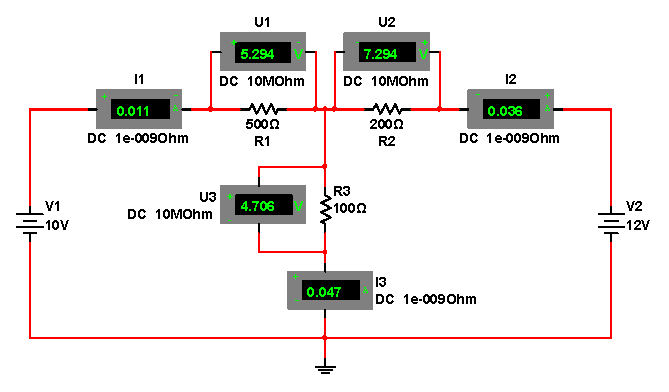
\includegraphics[width=.8\linewidth]{fig/exp1_result.eps}
                \caption{运行结果}
                \label{fig:1result}
            \end{figure}

            \newpage

            (2) 将$100\Omega$电阻改成 1N4009 的二极管(正极连接到A点上),自行建立表格,测量数据,测量计算分析KCL、KVL和叠加定理是否成立。
            \begin{figure}[htbp]
                \centering
                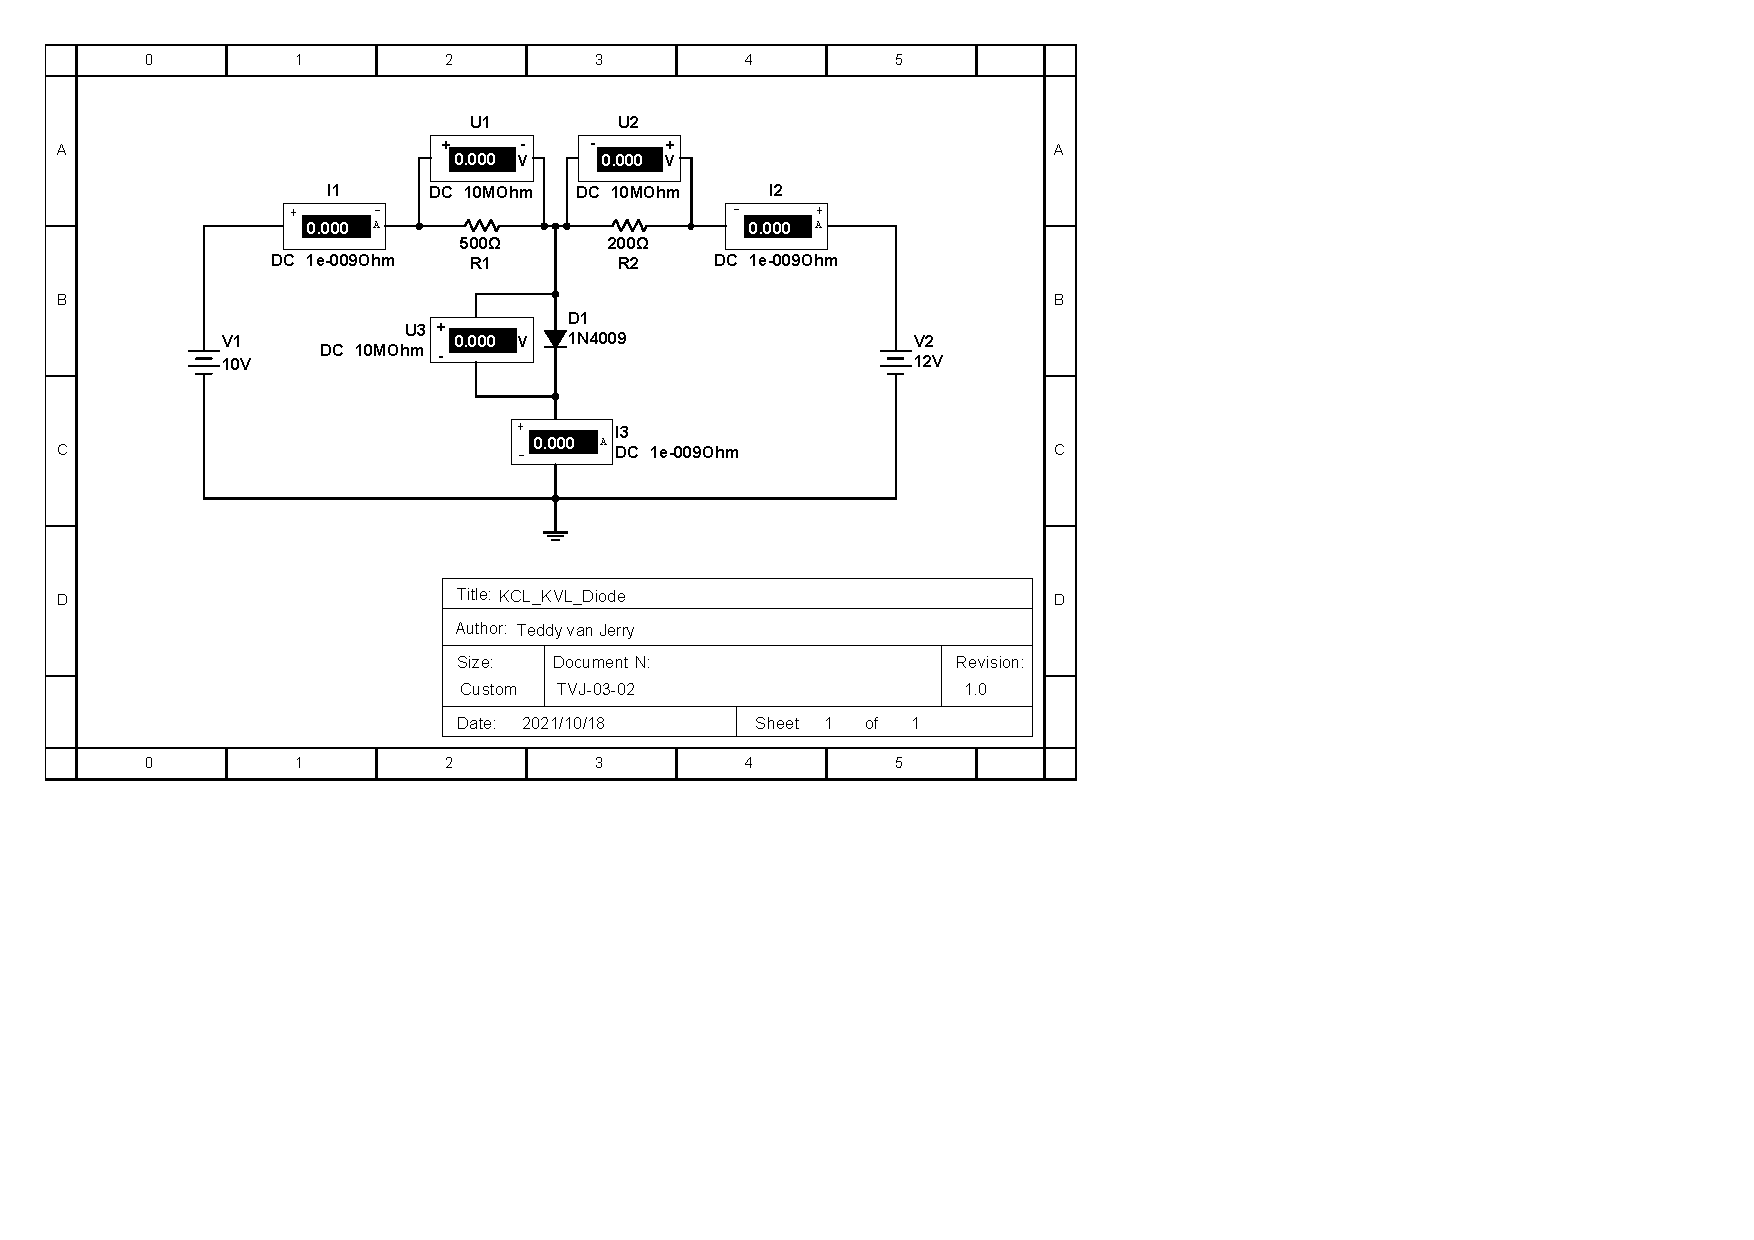
\includegraphics[width=.8\linewidth]{KCL_KVL_Diode.pdf}
                \caption{仿真电路图}
                \label{fig:2circuit}
            \end{figure}

            \begin{table}[htbp]
                \centering
                \begin{tabular}{ccccccc}
                    \toprule
                    \multirow{2}[4]{*}{状态} & \multicolumn{6}{c}{测量参数} \\
                    \cmidrule{2-7}\multicolumn{1}{c}{} & \multicolumn{1}{c}{$U_1$(V)} & \multicolumn{1}{c}{$U_2$(V)} & \multicolumn{1}{c}{$U_3$(V)} & \multicolumn{1}{c}{$I_1$(A)} & \multicolumn{1}{c}{$I_2$(A)} & \multicolumn{1}{c}{$I_3$(A)} \\
                    \midrule
                    $V_1$、$V_2$ 同时作用 & $9.001$ & $11.001$ & $0.999$ & $0.018$ & $0.055$ & $0.073$ \\
                    $V_1$ 单独作用 & $9.275$ & $-0.725$ & $0.725$ & $0.019$ & $-3.626\mathrm{m}$ & $0.725$ \\
                    $V_2$ 单独作用 & $-0.913$ & $11.087$ & $0.913$ & $-1.826\mathrm{m}$ & $0.055$ & $0.054$ \\
                    叠加结果  & $8.362$ & $10.362$ & $1.638$ & $0.017$ & $0.051$ & $0.779$ \\
                    \bottomrule
                \end{tabular}
                \caption{测量数据\protect\footnotemark}
                \label{tab:2data}
            \end{table}
            \footnotetext{此处也测量 $U_3$ 可以估算出二极管电阻随电流的变化关系。}

            \expexpect

            KCL 和 KVL 情况与第~\ref{subsec:exp1}~节(1)一致,
            而此时叠加原理将不满足,因为二极管不是线性元件。

            \emptyline
            \expanalyze

            \begin{equation}\label{eq:kcl_kvl_diode_result}
                \left\{
                    \begin{aligned}
                        & U_1+U_3=9.001+0.999=10.00\mathrm{V}=V_1 \\
                        & U_2+U_3=11.001+0.999=12.00\mathrm{V}=V_2 \\
                        & I_1+I_2=0.018+0.055=0.073\mathrm{A}=I_3
                    \end{aligned}
                \right.
            \end{equation}

            由式~\eqref{eq:kcl_kvl_diode_result}~可知,式~\eqref{eq:kcl_kvl_test}~成立,符合基尔霍夫定理预期。

            表~\ref{tab:2data}~中第一行与第四行不等,叠加原理不成立,与预期相符合。

            由文献\cite{diode_data_book}可知 1N4009 的正向电阻随着电流增大而减小,因此两个电源分别单独作用电流相加会大于两个电源同时作用,这与试验结果表~\ref{tab:2data}~中 $I_3$ 的表现相吻合。

            \emptyline
            \expsimulate

            \begin{figure}[htbp]
                \centering
                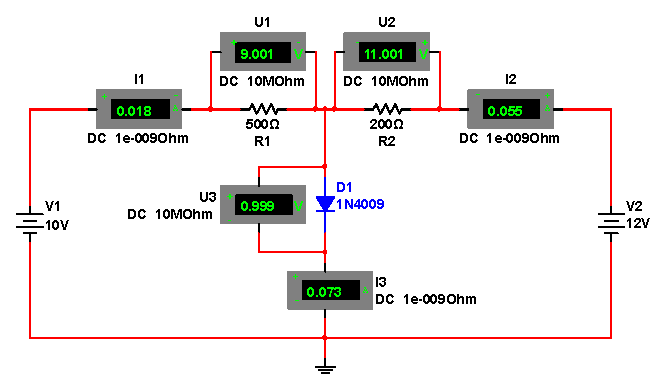
\includegraphics[width=.8\linewidth]{fig/exp2_result.eps}
                \caption{运行结果}
                \label{fig:2result}
            \end{figure}

        \newpage % 临时

        \subsection{设计电路,验证戴维南定理}
            (1) 将图~\ref{fig:1init}~中电阻$R_3$($100\Omega$)断开,测量电路A、B端口开路电压$U_{oc}$。

            \begin{figure}[htbp]
                \centering
                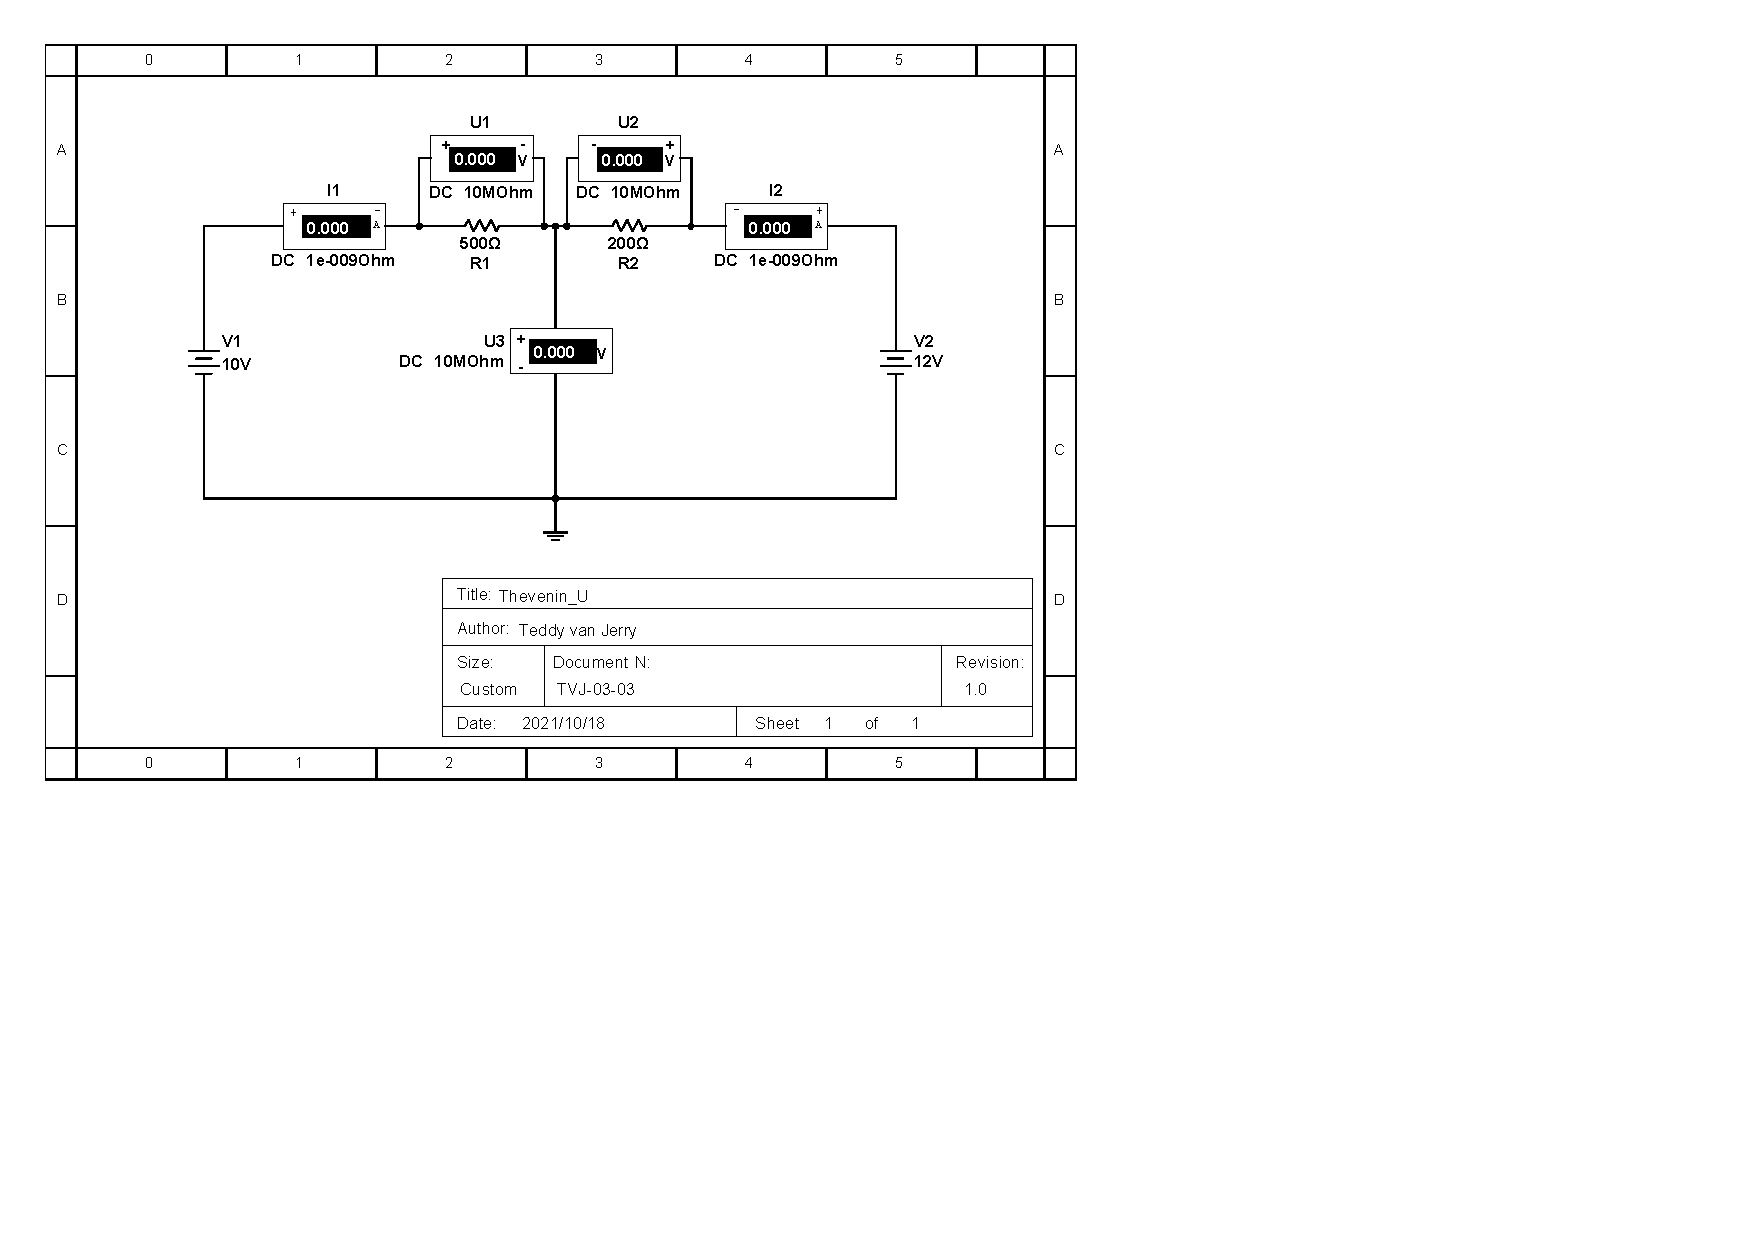
\includegraphics[width=.8\linewidth]{Thevenin_U.pdf}
                \caption{仿真电路图}
                \label{fig:3circuit}
            \end{figure}

            \expexpect

            由公式~\eqref{eq:thevenin}~可以得到其理论电压值 $11.4\mathrm{V}$。

            \emptyline
            \expsimulate

            \begin{figure}[htbp]
                \centering
                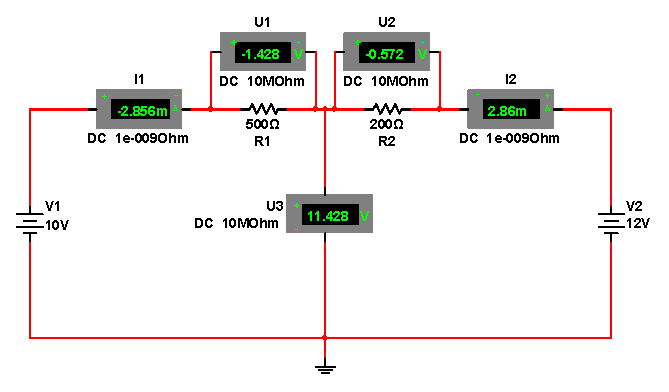
\includegraphics[width=.8\linewidth]{fig/exp3_result.eps}
                \caption{运行结果}
                \label{fig:3result}
            \end{figure}

            \newpage
        
            (2) 将电阻$R_3$短路,测得AB端口短路电流$I_{sc}$,计算等效电阻$R_o$。
            \begin{figure}[htbp]
                \centering
                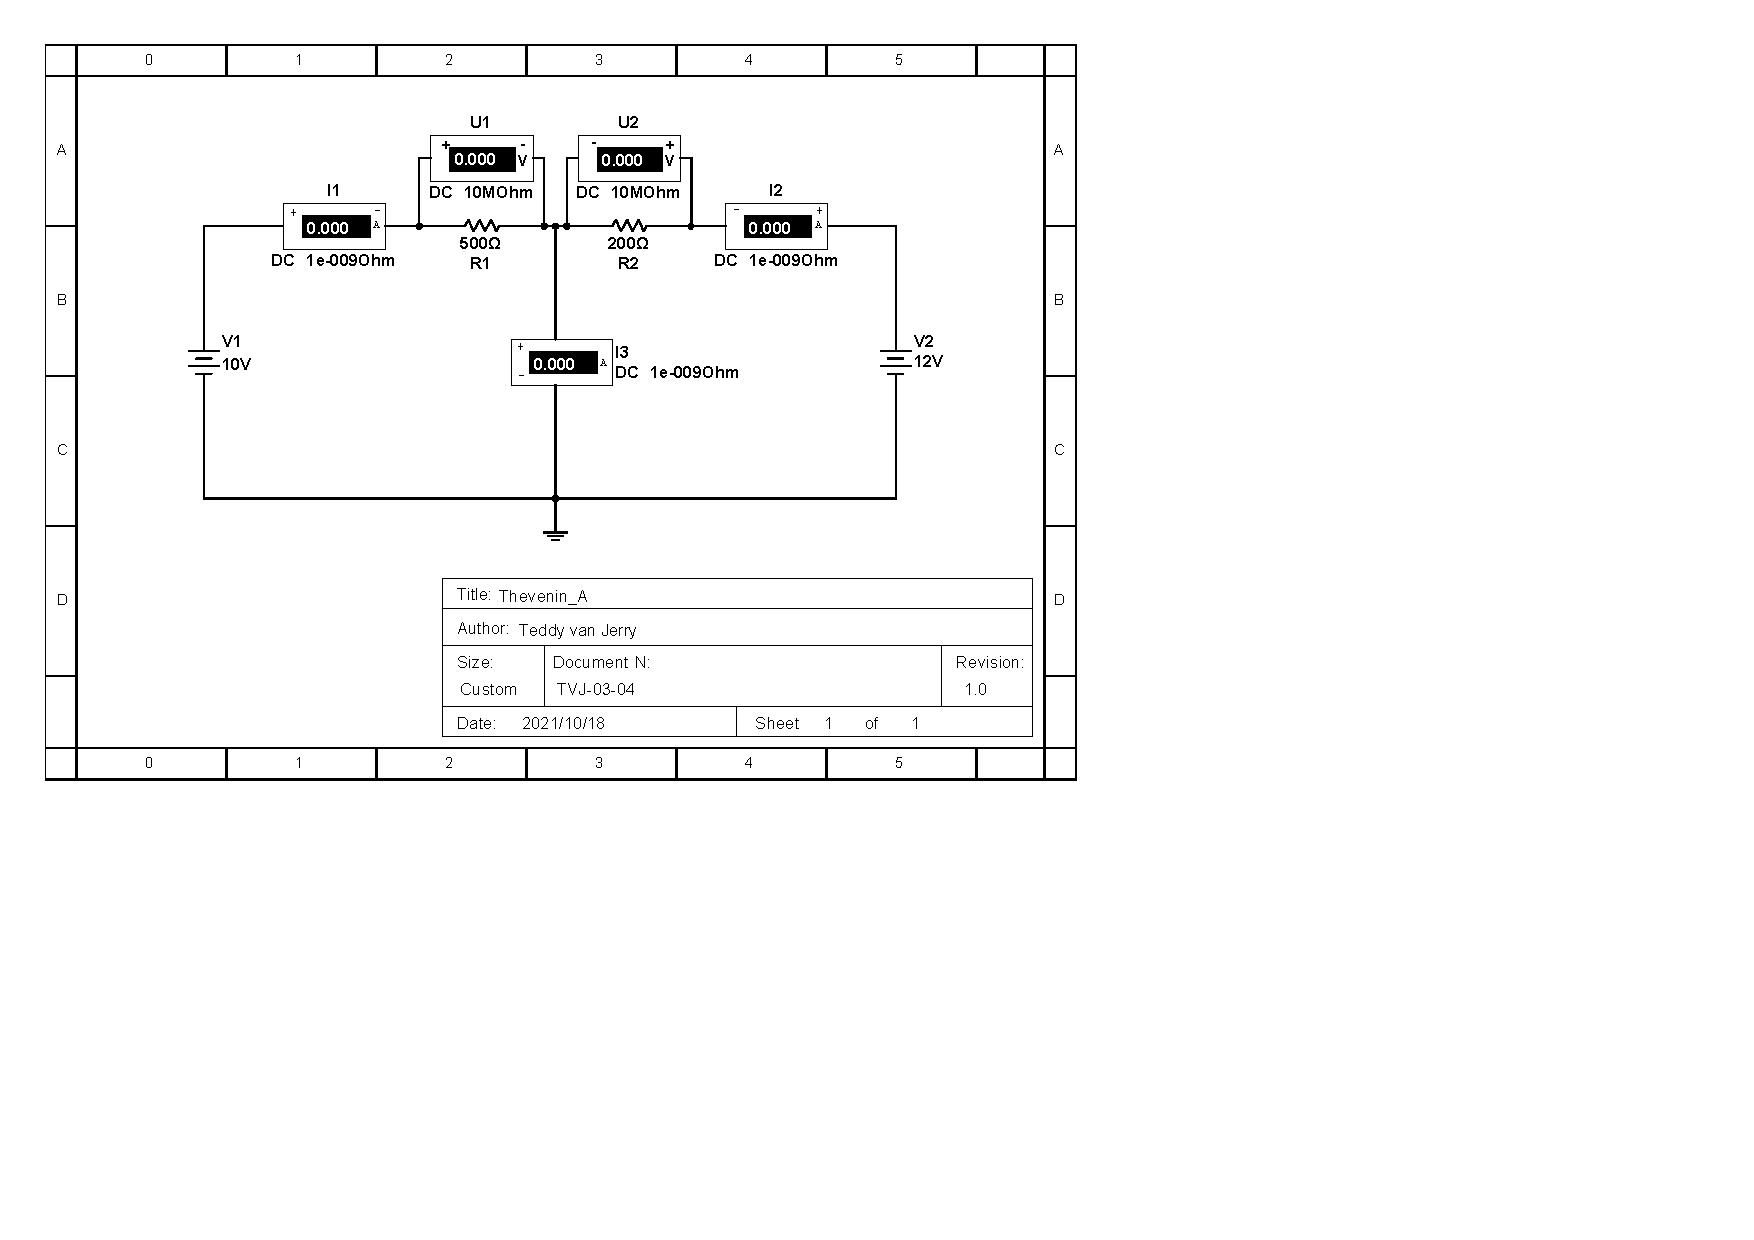
\includegraphics[width=.8\linewidth]{Thevenin_A.pdf}
                \caption{仿真电路图}
                \label{fig:4circuit}
            \end{figure}

            \expexpect

            由公式~\eqref{eq:thevenin}~可以得到其理论电压值约为 $11.4\mathrm{V}$,理论电阻值约为 $143\Omega$,理论电流为 $0.080\mathrm{A}$。

            \emptyline
            \expsimulate

            \begin{figure}[htbp]
                \centering
                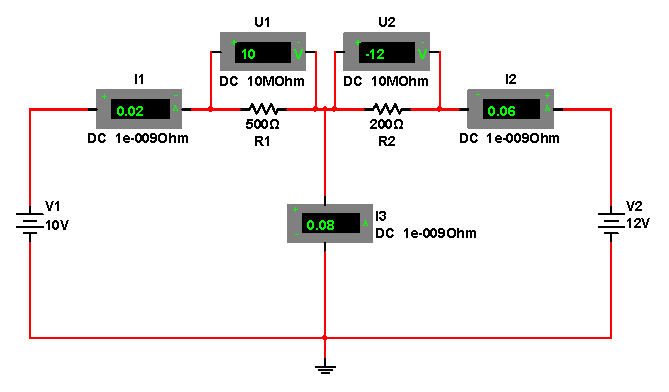
\includegraphics[width=.8\linewidth]{fig/exp4_result.eps}
                \caption{运行结果}
                \label{fig:4result}
            \end{figure}

            \newpage
            
            (3) 建立等效电路,验证戴维南定理。
            \begin{figure}[htbp]
                \centering
                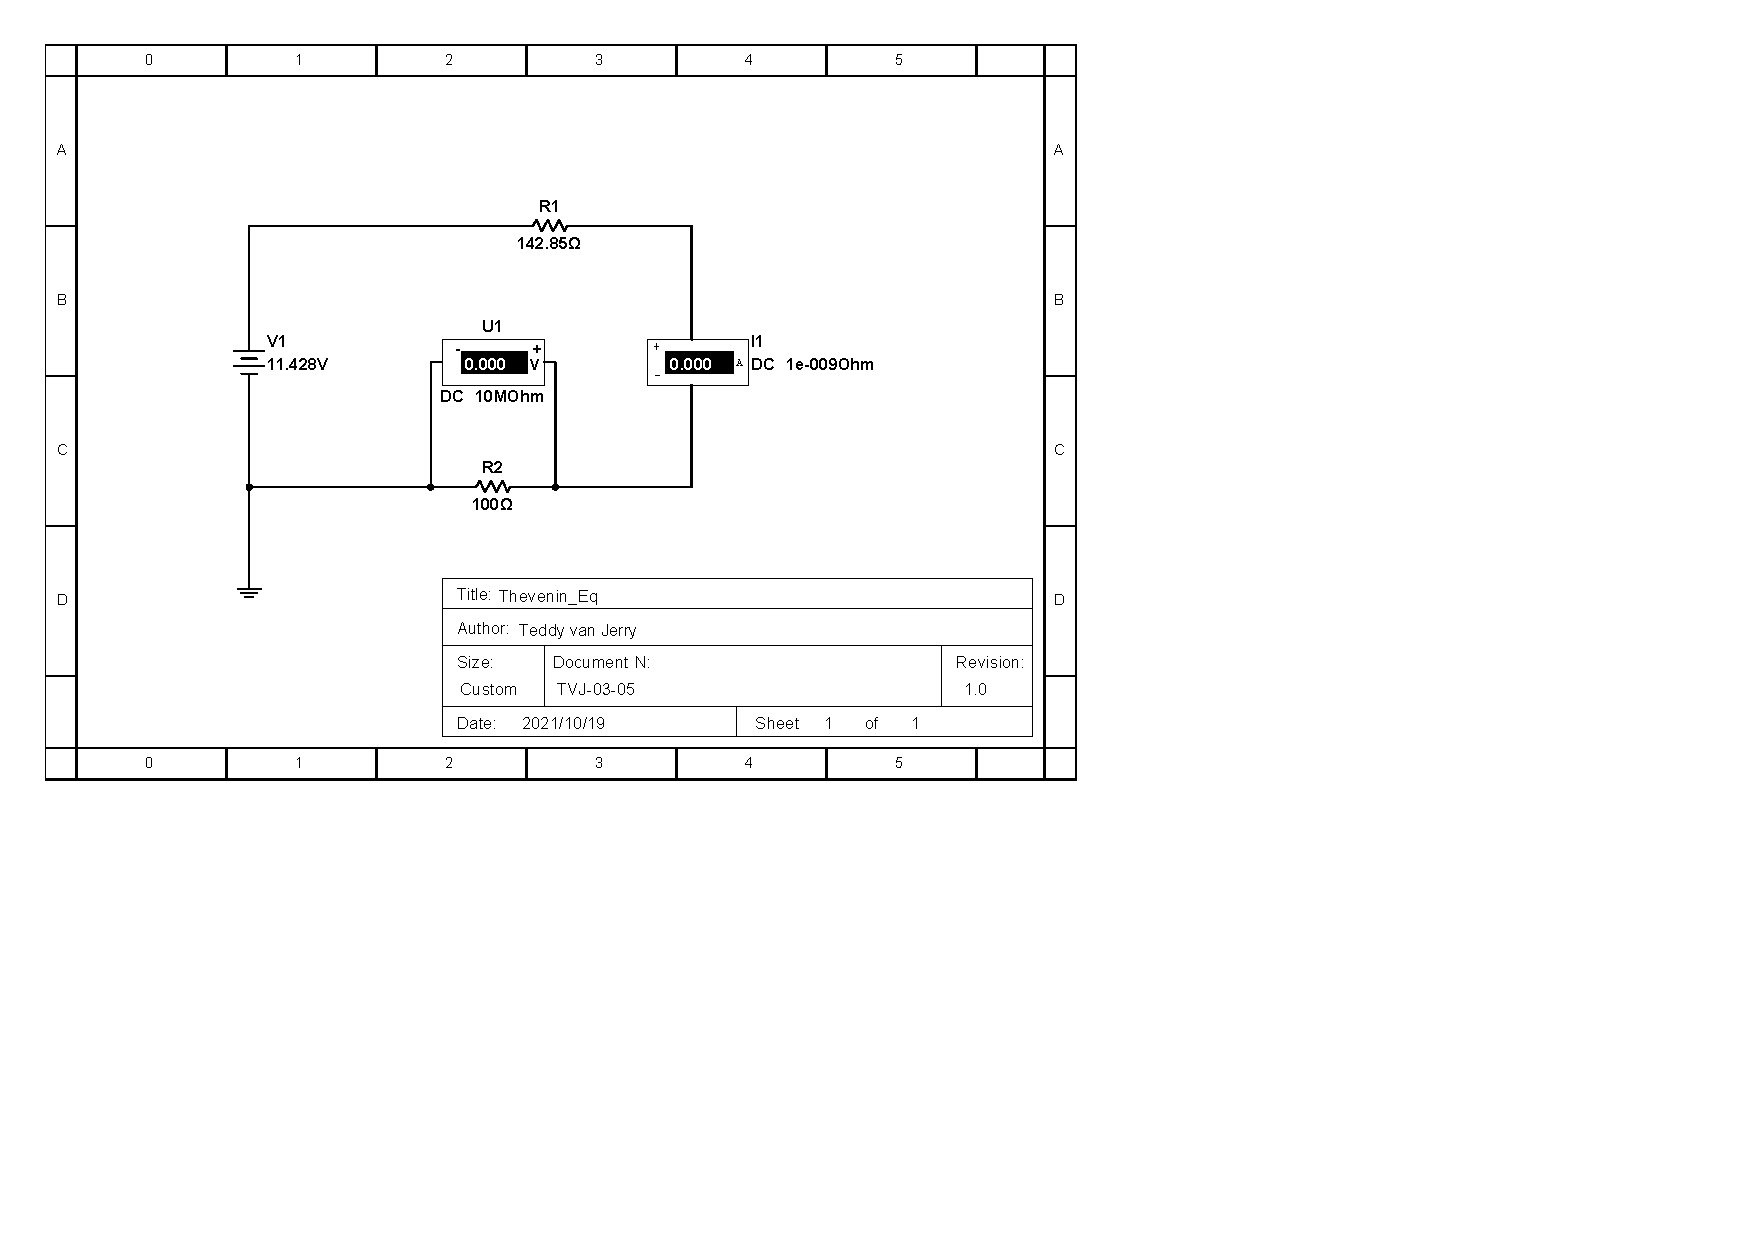
\includegraphics[width=.8\linewidth]{Thevenin_Eq.pdf}
                \caption{仿真电路图}
                \label{fig:5circuit}
            \end{figure}

            \begin{table}[htbp]
                \centering
                \begin{tabular}{ccccc}
                    \toprule
                    $U_{OC}$(V) & $I_{SC}$(A) & $R_o$($\Omega$) & $U$(V) & $I$(A) \\
                    \midrule
                    $11.428$ & $0.08$ & $142.85$ & $4.706$ & $0.047$ \\
                    \bottomrule
                \end{tabular}
                \caption{实验数据}
                \label{tab:4data}
            \end{table}
            
            \expexpect

            由公式~\eqref{eq:thevenin}~可以得到其理论电压值约为 $11.4\mathrm{V}$,理论电阻值约为 $143\Omega$。

            \emptyline
            \expanalyze

            理论计算值与实验值一致,电压源并联公式~\eqref{eq:thevenin}~成立。

            表~\ref{tab:4data}~中负载电压和电流与表~\ref{tab:1data}~中一致,与戴维南定理预期符合。

            \newpage % 此系调整此页板式特别添加
            \expsimulate

            \begin{figure}[htbp]
                \centering
                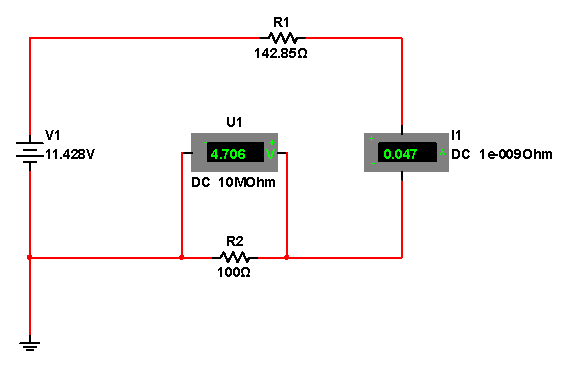
\includegraphics[width=.8\linewidth]{fig/exp5_result.eps}
                \caption{运行结果}
                \label{fig:5result}
            \end{figure}   

    \section{实验使用仪器设备(使用软件)}

        我使用 Multisim 14.0(我自己安装了新版本,没有使用学校的 13.0 版本),保存文件后缀为 \texttt{ms14}。

        报告撰写使用 Visual Studio Code 配合 \LaTeXe。

        \begin{figure}[htbp]
            \centering
            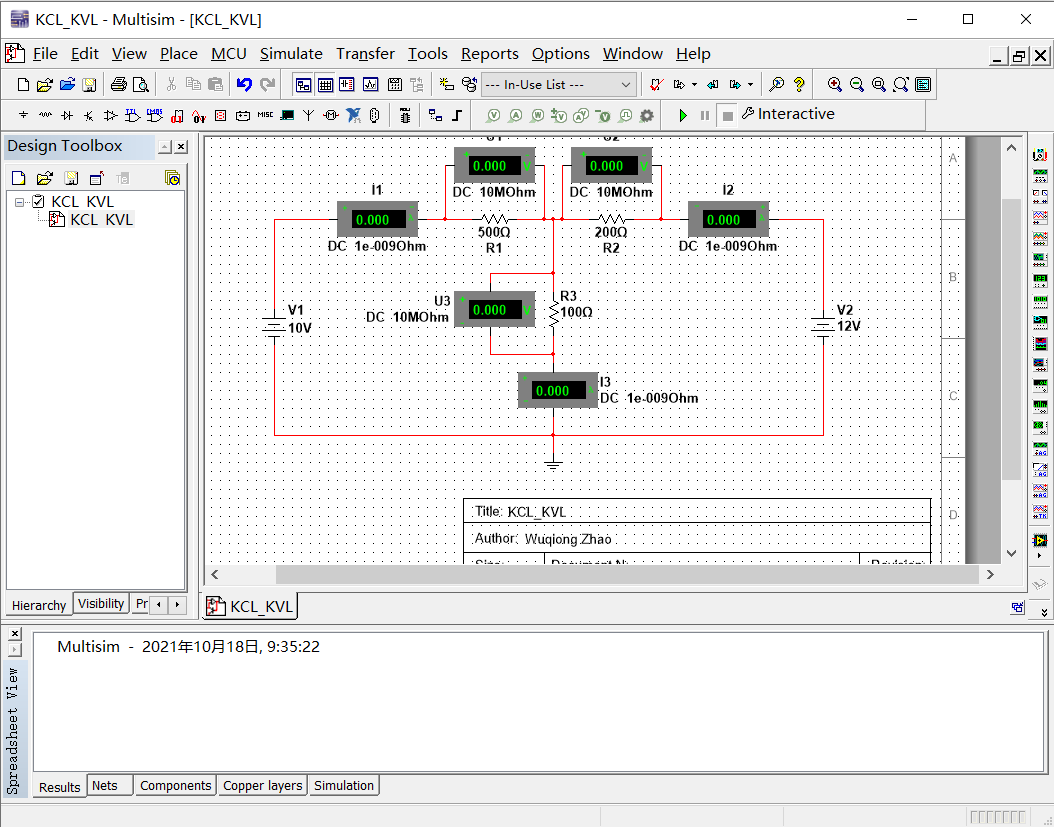
\includegraphics[width=.75\linewidth]{fig/Multisim_KCL_KVL_Design.png}
            \caption{Multisim 14.0 设计界面}
            \label{fig:multisim_design_window}
        \end{figure}

    \newpage

    \section{实验总结}

        实验结果均符合预期,没有明显的误差问题。实验中的问题与思考包括电流表的内外接法(第~\ref{subsec:exp1}~节(1))、二极管叠加效果的分析(第~\ref{subsec:exp1}~节(2))。

        首次使用 Multisim,根据文献\cite{teaching_schedule}指导进行非常顺利,
        不过我试图添加 Title Block 的时候遇到了问题,通过资料\cite{multisim_help}找到了解决方案。

        此外,我也编写了实验报告 \LaTeX 模板,创建了 \texttt{SEU-Circuit-Report.cls},提升了 \LaTeX 编写的技能。

    % 打印参考文献
    \printbibliography

    \newpage

    \section*{附录:\LaTeX 模板使用说明}

        报告模板下载:\url{https://github.com/Teddy-van-Jerry/SEU_Circuit_Report}。

        \LaTeX 文档编译使用 \texttt{XeLaTeX + Biber}。

        文档信息只需要修改以下部分,就可以自动生成封面页即对应内容

        \begin{lstlisting}[language=TeX]
%% 使用实验报告模板类(字体大小 12pt 最适合)
\documentclass[12pt]{SEU-Circuit-Report}

%%%%%%%%%%%%%%%%%%%% 报告基本信息 %%%%%%%%%%%%%%%%%%%%
\expno{3} % 实验序号
\expname{应用Multisim软件工具设计电路验证网络定理} % 实验名称
\exphouse{TVJ Group} % 学院
\expmajor{\LaTeX\ Design} % 专业
\expauthor{Teddy van Jerry} % 姓名
\expID{123456} % 学号
\explab{} % 实验室
\expgroup{} % 实验组别
\expmates{} % 同组人员
\expdate{2021年10月19日} % 实验日期
\expgrade{} % 成绩评定
\exptutor{Mentor Name} % 评阅老师
%%%%%%%%%%%%%%%%%%%%%%%%%%%%%%%%%%%%%%%%%%%%%%%%%%%%
        \end{lstlisting}

        Word 版报告模板中的电路图以 Visio 格式内嵌,右击选择打开,
        再导出为 PDF,可以再使用 Acrobat Pro 裁去白边框(Remove White Margin)并导出成 \texttt{eps} 格式。

        在报告中插入 Multisim 矢量图需要先将 Multisim 选中内容复制到 Word,再将 Word 当作压缩包打开,在 \texttt{word/media} 中找到对应的 \texttt{emf} 图片,在~\url{https://cloudconvert.com/emf-to-eps}~或~\url{https://www.aconvert.com/image/emf-to-eps}~中转换成~\texttt{eps}~即可插入。

\end{document}
